% !TeX encoding = UTF-8
    % !TEX root = ./presentation.tex
    % !TEX spellcheck = pt_BR
    
    
    
    \subsection{{\it Field-Programmable Logic Device} (FPGA) e Recursos}
    
    	\begin{frame}{\textit{Field-Programmable Logic Device} (FPGA)}{Hardware - Visão Geral}
    		\begin{itemize}
    			\setlength\itemsep{0.8em}
                \item FPGAs eram utilizados unicamente na protitipação ASIC.
                
                \item Mas com a \textbf{elevação do custo} de pesquisa, \design, desenvolvimento e teste de um novo produto
                \begin{itemize}
                    \setlength{\itemsep}{0.5em}
                    \item Interessou-se na utilização de FPGAs \cite{Mei2000};
                    \item Vantagens em termos de flexibilidade de projeto.
                \end{itemize}
                
                \item Entretanto \cite{Sass2010}
                \begin{itemize}
                    \setlength{\itemsep}{0.5em}
                    \item + Configurar um \hardware\ reconfigurável é uma tarefa fácil;
                    
                    \item - \textbf{Criar um \design\ de \hardware\ inicial não é}.
                \end{itemize}
                    \bigskip
    			\item Internamente:
    			\begin{itemize}
                    \setlength{\itemsep}{0.5em}
    				\item Consiste num \textbf{arranjo de blocos lógicos} e \textbf{canais de roteamento}.
    
    				\item Significa que é capaz de alterar seus caminhos de dados/fluxos \textbf{habilitando/desabilitando módulos} \cite{moreira2008}.
    			\end{itemize}
    		\end{itemize}
    	\end{frame}
    
    
    	\begin{frame}{\textit{Field-Programmable Logic Device} (FPGA)}{Hardware - Visão Geral}
    		\begin{figure}[h]
    			\centering
    			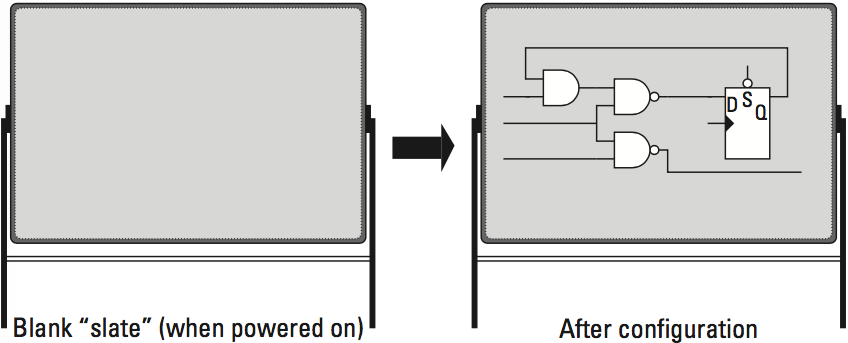
\includegraphics[width=1\textwidth]{img/rt-board.png}
    			\label{fig:quadro}
                \caption{``FPGA é um \textit{quadro negro} que pode ser \textit{desenhado} qualquer circuito digital''.}
    		\end{figure}
    	\end{frame}
    
    \begin{frame}{\textit{Field-Programmable Logic Device} (FPGA)}{Hardware - Estrutura Interna} 
    \vspace{-1em}
    \begin{figure}[h] \centering
        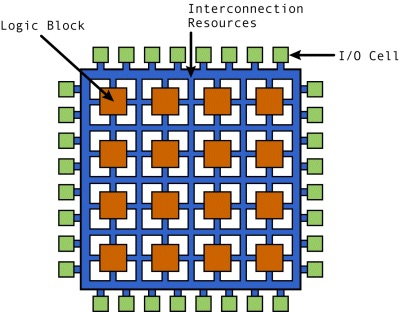
\includegraphics[width=0.7\textwidth]{img/rt-arch_fpga.jpg}
        \vspace{-0.5em}
        \caption{Exemplo da arquitetura internas de um FPGA. Fonte: \url{http://www.eetimes.com/document.asp?doc_id=1274496}. Acesso: 30/05/2017.}
    \end{figure}
    \pdfnote{Tornando-o um dos (CI) MAIS densos existente.}
    \end{frame}
    
    	\begin{frame}{\textit{Field-Programmable Logic Device} (FPGA)}{Hardware - Estrutura Interna} 
            \vspace{-0.8em}
    		\begin{figure}[H]
    			\centering
    			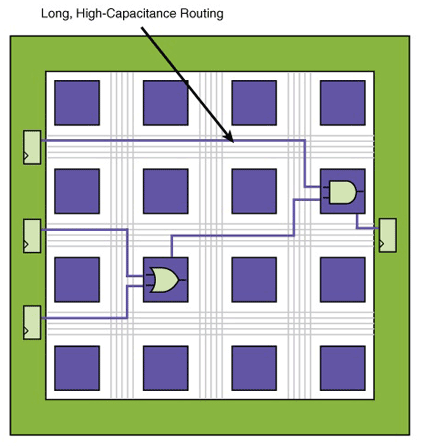
\includegraphics[width=0.56\textwidth]{img/fpga/exemploInicial.png}
                \vspace{-0.5em}
    			\caption{Demonstração mais complexa de síntese.}
    		\end{figure}
    	\end{frame}
    
    	\begin{frame}{\textit{Field-Programmable Logic Device} (FPGA)}{Hardware - Estrutura Interna}
            \vspace{-1em}
    		\begin{figure}[h]
    			\centering
    			\includegraphics[width=0.6\textwidth]{img/fpga/exemploFinal.png}
                \vspace{-1em}
    			\caption{Exemplo de roteamento interno complexo no FPGA.}
    			\label{fig:exemploFinal}
    		\end{figure}
    	\end{frame}
    
    
    \begin{frame}{\textit{Field-Programmable Logic Device} (FPGA)}{Hardware - Estrutura Interna}
    \vspace{-1em}
    \begin{figure}[p]
        \centering
        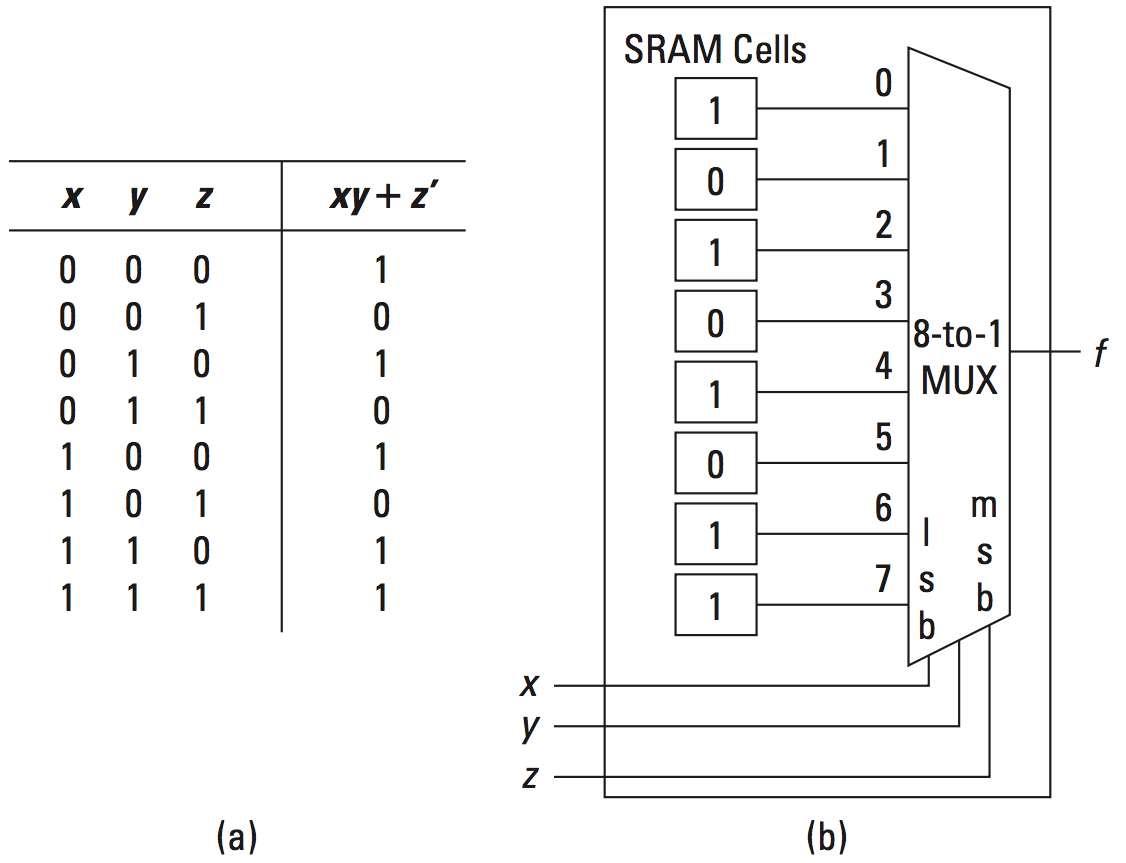
\includegraphics[width=0.74\textwidth]{img/fpga/funcao-geradora.png}
        \vspace{-0.7em}
        \caption{Gerador de Função. a) tabela verdade e b) Look-Up Table (LUT) com Flip-flops para armazenamento e execução como um multiplexador.}
        \label{fig:funcao-geradora}
    \end{figure}
    \end{frame}
    
    
    	\begin{frame}{\textit{Field-Programmable Logic Device} (FPGA)}{Software - Altera Quartus II}
            \vspace{-1em}
    		\begin{figure}[p]
    			\centering
    			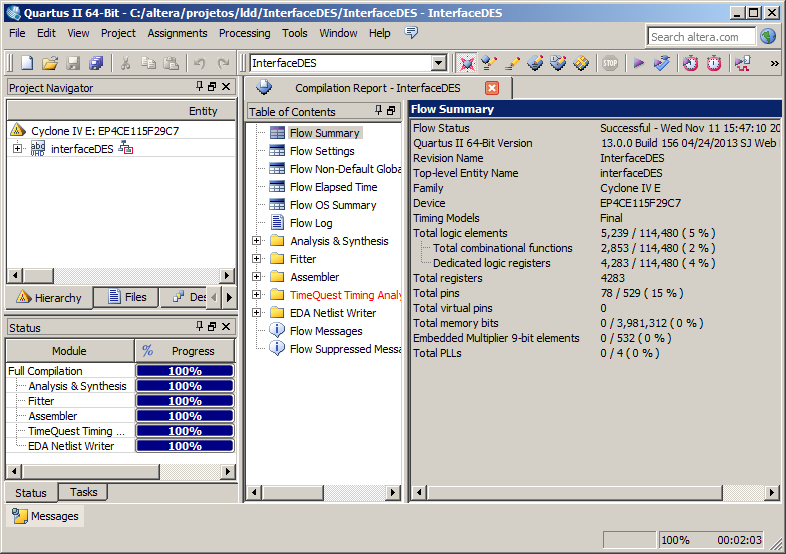
\includegraphics[width=0.87\textwidth]{img/fpga/altera.png}
                \vspace{-0.8em}
    			\caption{Altera Quartus II.}
    			\label{fig:alteraquartus}
    		\end{figure}
    	\end{frame}
    
    
    
    \begin{frame}{\textit{Field-Programmable Logic Device} (FPGA)}{Codificação} 
    \vspace{-0.7em}
    \begin{itemize}
        \setlength\itemsep{1.3em}
        \item A implementação na placa FPGA é feita por:
        \begin{itemize}
            \setlength\itemsep{0.5em}
            \item Linguagens de descrição chamadas de \textbf{Linguagens de Descrição de \textit{Hardware} (HDL)}
            \begin{itemize}
                \item São algumas linguagens: VHDL, Verilog, ABEL, etc..
            \end{itemize}
            
            \item Ou por meio do desenvolvimento de \textbf{diagramas esquemáticos com ferramentas gráficas assistidas pelo computador}.
            
            \item Hoje, também é possível escrever por meio de \textbf{linguagens de alto nível} para como Handel-C, C-like ou mesmo o SystemC.
        \end{itemize}
        
        \item Alguns conceitos de fundamentais sobre linguagens de descrição de \textit{hardware}:
        \begin{itemize}
            \setlength\itemsep{0.5em}
            \item Estas linguagens permitem por exemplo \textit{loops} infinitos ou portas lógicas com inúmeras entradas;
            
            \item Essas são possível serem descritas em \textit{software} mas impossível de implementar em \textit{hardware}.
        \end{itemize}
    \end{itemize}
    \end{frame}
    
    \begin{frame}{\textit{Field-Programmable Logic Device} (FPGA)}{Codificação - \textit{Hardware Description Language} (HDL)} 
    \vspace{-1em}
    \begin{itemize}
        \setlength{\itemsep}{1.0em}
        \item \textbf{Classes de linguagens} de computação usados para \textbf{descrever formalmente um circuito eletrônico}.
        \begin{itemize}
            \item Pois possui detalhação altíssima do \hardware.
        \end{itemize} 
        
        \item Descreve o \cite{Sass2010}
        
        \begin{itemize}
            \item \textbf{Comportamento temporal}; ou a 
            \item \textbf{Estrutura de circuito espacial} de um sistema eletrônico.
        \end{itemize}
        
        \item Vantagens \cite{Smith1998}
        \begin{itemize}
            \item Pode-se \textbf{alterar} o código HDL, \textbf{e sintetizar no mesmo dispositivo} para testar;
            \item \textbf{Quantas vezes forem necessárias}, \textbf{sem custo adicional}.
        \end{itemize}
        
        \item Desvantagem
        \begin{itemize}
            \item - \textbf{Nível elevado de complexidade} de programação  \cite{Choi2016};
            \item + Existe outras linguagens disponíveis para uso \cite{Sass2010}. 
        \end{itemize}
    \end{itemize}
    \end{frame}
    
    
    
    \begin{frame}{\textit{Field-Programmable Logic Device} (FPGA)}{Codificação - \textit{Hardware Description Language} (HDL) - VHDL}
    \begin{itemize}
    \setlength\itemsep{1.3em}
    \item Linguagem para descrever o \textbf{comportamento} e \textbf{estrutura} de um sistema digital.
    
    \item A abreviatura de VHDL significa \textit{\underline{VHSIC Hardware Description Language}}
    \begin{itemize}
    \item Sendo que VHSIC significa \textit{\underline{Very High Speed Integrated Circuit}}.
    \end{itemize}
    
    \item Ou seja, seu nome em português é \textbf{Linguagem de Descrição de \textit{Hardware} de Circuitos Integrados com Altíssima Velocidade}.
    
    \item Ela tem propriedades suficientes para ser \textbf{independente tecnologicamente} \cite{Roth1998}.
    \end{itemize}
    \end{frame}
    
    
    \begin{frame}{\textit{Field-Programmable Logic Device} (FPGA)}{Software - Programação por Linguagem de Descrição}
    \vspace{-1em}
    \begin{figure}[p]
        \centering
        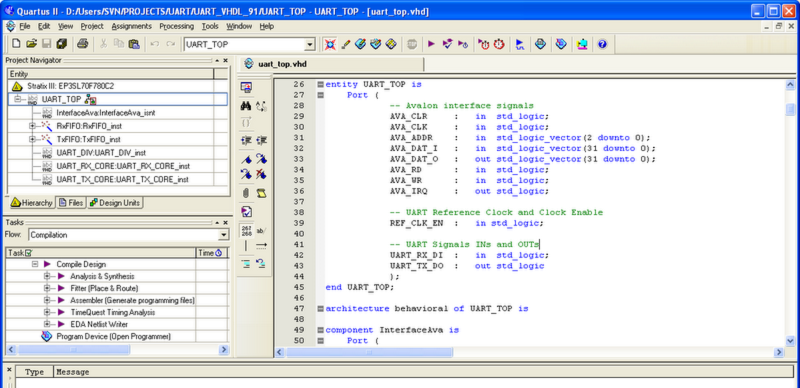
\includegraphics[width=1\textwidth]{img/fpga/software_quartus_vhdl.png}
        \caption{Portos de uma interface UART usando VHDL.}
        \label{fig:alteraquartus_portas}
    \end{figure}
    \end{frame}
    
    
    
    
    	\begin{frame}{\textit{Field-Programmable Logic Device} (FPGA)}{Codificação - Portas Lógicas}
            \vspace{-1em}
    		\begin{figure}[p]
    			\centering
    			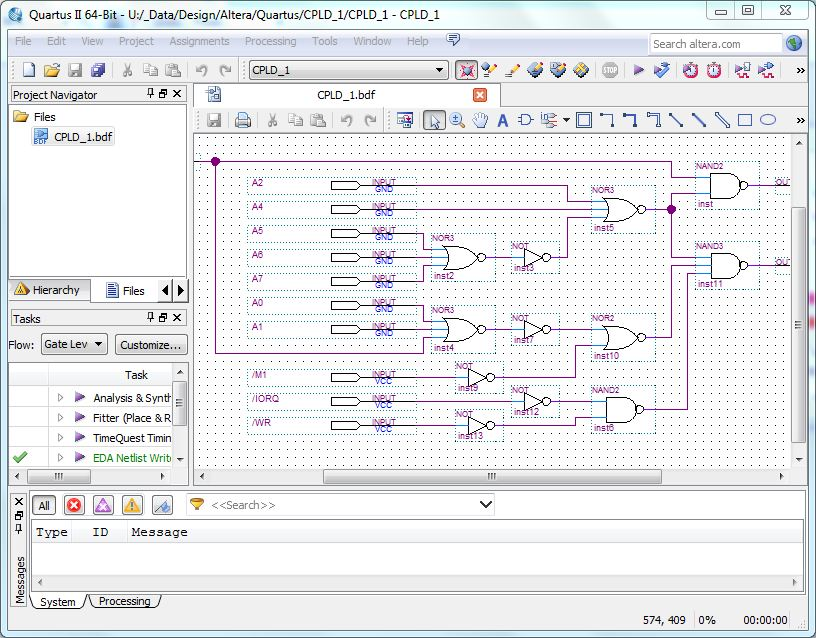
\includegraphics[width=0.78\textwidth]{img/fpga/software_quartus_portas.jpg}
                \vspace{-0.8em}
    			\caption{Projeto com assistência computacional usando portas lógicas.}
    			\label{fig:alteraquartus_portas1}
    		\end{figure}
    	\end{frame}
    
    	\begin{frame}{\textit{Field-Programmable Logic Device} (FPGA)}{Codificação - Portas Lógicas}
            \vspace{-1em}
    		\begin{figure}[p]
    			\centering
    			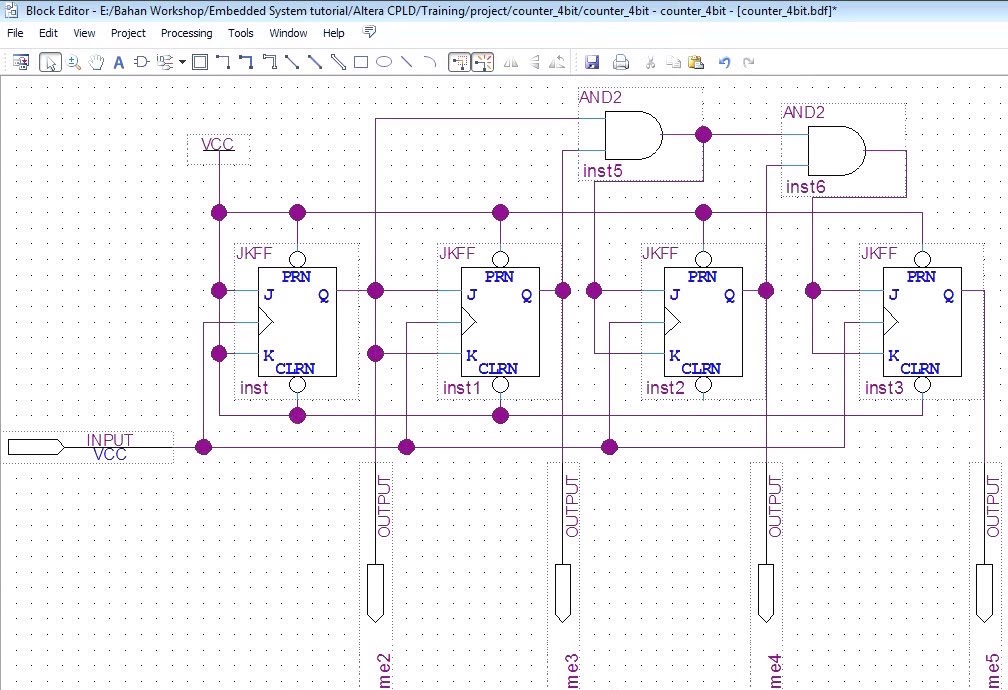
\includegraphics[width=0.9\textwidth]{img/fpga/software_quartus_portas2.jpg}
                \vspace{-0.7em}
    			\caption{Projeto Contador 4-bit usando portas lógicas.}
    			\label{fig:alteraquartus_portas2}
    		\end{figure}
    	\end{frame}
    
    	\begin{frame}{\textit{Field-Programmable Logic Device} (FPGA)}{Software - Exemplo de Programação}
    		\begin{figure}[p]
    			\centering
    			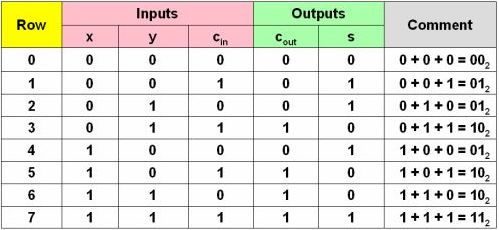
\includegraphics[width=1\textwidth]{img/fpga/adder-table.jpg}
    			\caption{Somador Completo.}
    			\label{fig:somador_completo}
    		\end{figure}
    	\end{frame}
    
    	\begin{frame}{\textit{Field-Programmable Logic Device} (FPGA)}{Software - Exemplo de Programação}
    		\begin{figure}[p]
    			\centering
    			
\includegraphics[width=0.77\textwidth]{img/fpga/adder.png}
    			\caption{Representação do Somador Completo em Portas Lógicas.}
    			\label{fig:somador_completo_pl}
    		\end{figure}
    	\end{frame}
    
    	\begin{frame}[fragile]{\textit{Field-Programmable Logic Device} (FPGA)}{Software - Exemplo de Programação}
        \vspace{-1.1em}
        \begin{center}
            \begin{minipage}{10cm}
                \begin{minted}[
                gobble=0,
                linenos,
                fontsize=\small,
                baselinestretch=1.1,
                numbersep=5pt,
                frame=lines]{vhdl}
library ieee;
use ieee.std_logic_1164.all;

entity fadder is port (
    a, b : in std_logic;
    cin  : in std_logic;
    sum  : out std_logic;
    cout : out std_logic);
end fadder;

architecture beh of fadder is 
begin
    sum <= a xor b xor cin;
    cout <= (a and b) or (b and cin) or (a and cin);
end beh;
                \end{minted}
            \end{minipage}
        \end{center}
    \end{frame}
    
    
    	\begin{frame}{\textit{Field-Programmable Logic Device} (FPGA)}{Software - Exemplo de Programação}
            \vspace{-1em}
    		\begin{figure}[p]
    			\centering
    			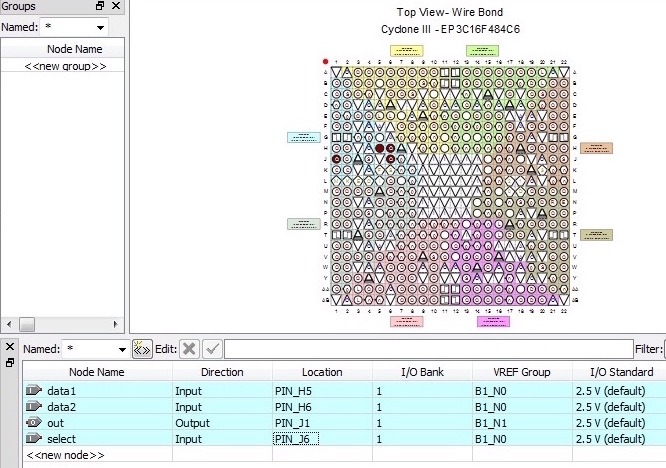
\includegraphics[width=0.89\textwidth]{img/fpga/software_quartus_pin.jpg}
                \vspace{-0.8em}
    			\caption{Pin Planner.}
    			\label{fig:alteraquartus_pinagem}
    		\end{figure}
    	\end{frame}
    
    	\begin{frame}%{FPGA - Software - IDE de Desenvolvimento}
            \vspace{-0.5em}
    		\begin{figure}[p]
    			\centering
    			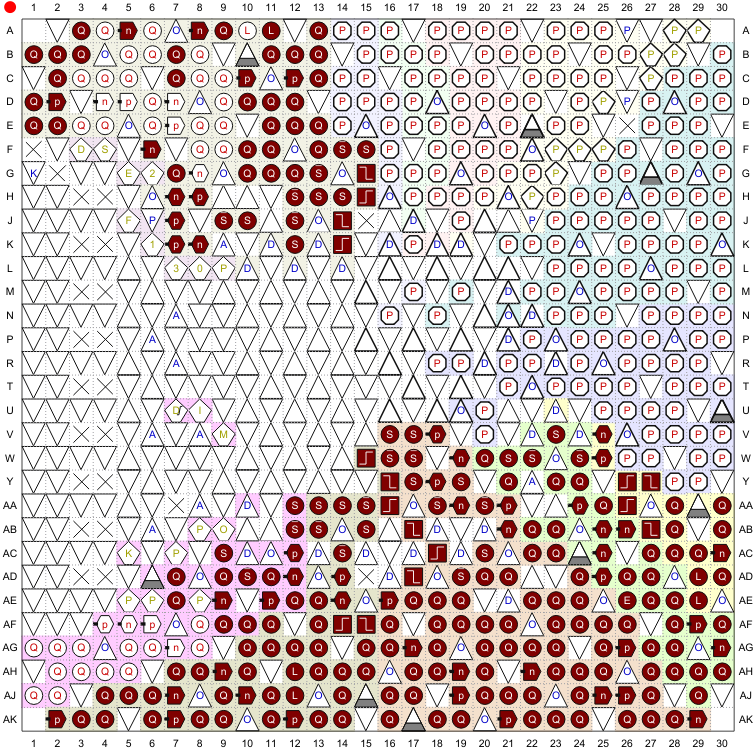
\includegraphics[width=0.75\textwidth]{img/fpga/pinplanner.png}
                \vspace{-0.8em}
    			\label{fig:pinplanner}
    		\end{figure}
    	\end{frame}
    
    	\begin{frame}{\textit{Field-Programmable Logic Device} (FPGA)}{Software - Exemplo de Programação}
        \vspace{-0.5em}
    		\begin{figure}[p]
    			\centering
    			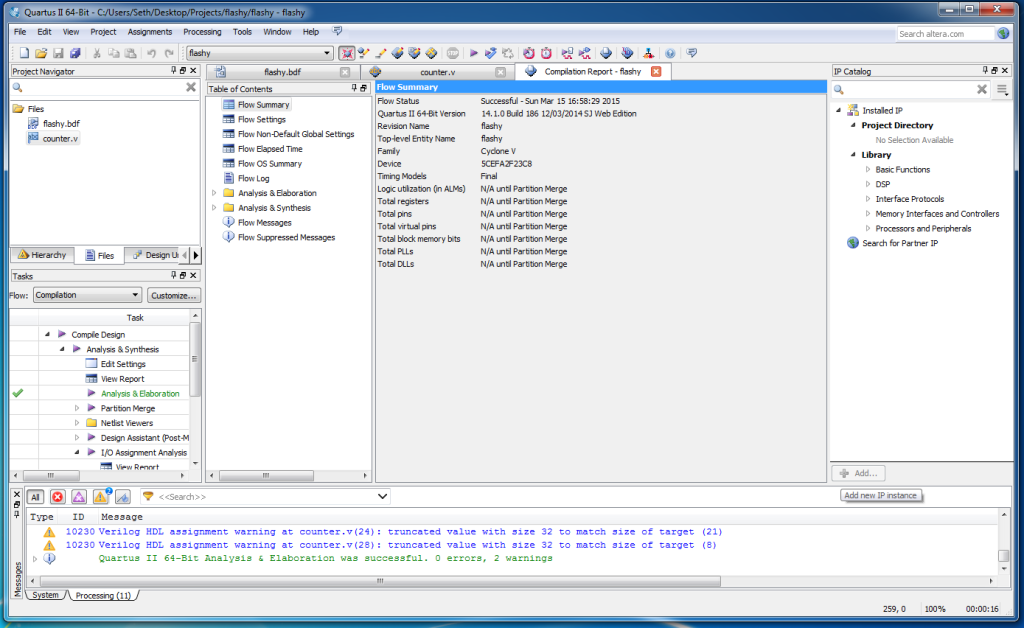
\includegraphics[width=0.95\textwidth]{img/fpga/software_quartus_compilation0.png}
                \vspace{-0.5em}
    			\caption{Início de síntese de um projeto.}
    			\label{fig:alteraquartus_comp0}
    		\end{figure}
    	\end{frame}
    
    	\begin{frame}{\textit{Field-Programmable Logic Device} (FPGA)}{Software - Exemplo de Programação}
    		\begin{figure}[p]
    			\centering
    			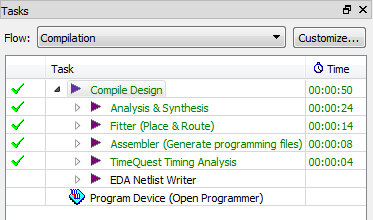
\includegraphics[width=0.9\textwidth]{img/fpga/software_quartus_compilation1.png}
    			\caption{Término de síntese de um projeto.}
    			\label{fig:alteraquartus_comp1}
    		\end{figure}
    	\end{frame}
    
    	\begin{frame}{\textit{Field-Programmable Logic Device} (FPGA)}{Software - Exemplo de Programação}
    		\begin{figure}[p]
    			\centering
    			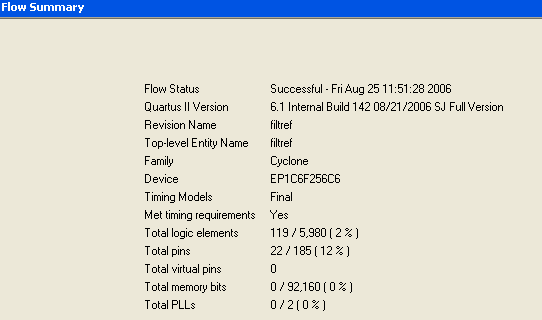
\includegraphics[width=0.9\textwidth]{img/fpga/software_quartus_compilation2.png}
    			\caption{Relatório de compilação final.}
    			\label{fig:alteraquartus_comp2}
    		\end{figure}
    	\end{frame}
    
    	\begin{frame}{\textit{Field-Programmable Logic Device} (FPGA)}{Software - Exemplo de Programação}
            \vspace{-0.5em}
    		\begin{figure}[p]
    			\centering
    			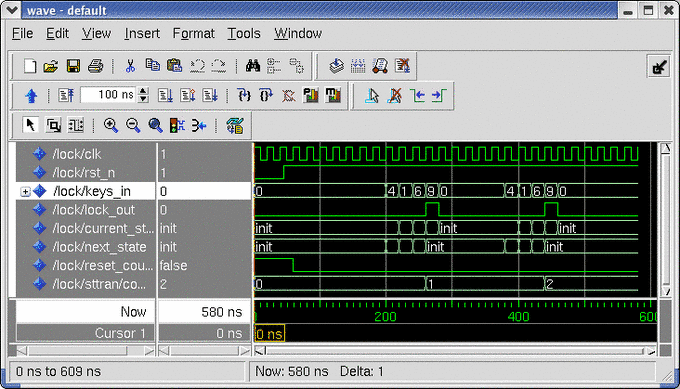
\includegraphics[width=1\textwidth]{img/fpga/modelsim.png}
                \vspace{-0.5em}
    			\caption{ModelSim.}
    			\label{fig:modelsim}
    		\end{figure}
    	\end{frame}
    
    \begin{frame}%{\textit{Field-Programmable Logic Device} (FPGA)}{Software - Exemplo de Programação}
    \vspace{-0.6em}
    \begin{figure}[p]
        \centering
        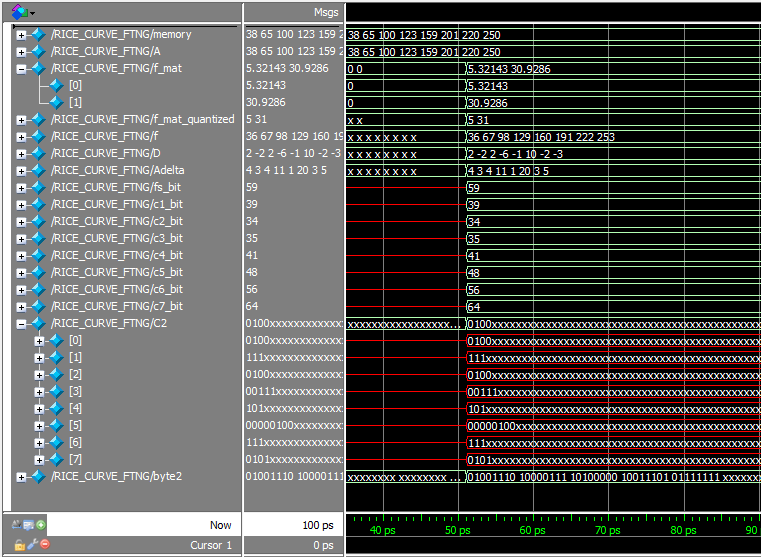
\includegraphics[width=0.97\textwidth]{img/fpga/waveform.png}
        \vspace{-0.6em}
        \caption{Waveforms.}
        \label{fig:waveform}
    \end{figure}
    \end{frame}
    
    \begin{frame}{\textit{Field-Programmable Logic Device} (FPGA)}{Codificação - \textit{High-Level Synthesis} (HLS)} 
    \vspace{-1em}
    \begin{itemize}
        \setlength{\itemsep}{0.9em}
        \item Sintetizam códigos de alto nível para HDLs \cite{Choi2016} \cite{Trevett2008}
        \begin{itemize}
            \setlength{\itemsep}{1.2em}
            \item \textbf{Reduzir} os longos ciclos do \textbf{processo de \design}\ de \hardware; e ainda
            \item Traz \textbf{melhoria em performance e eficiência energética};
            \item Entrega um bom HDL.
        \end{itemize}
        
        \pdfnote{bib \textit{multi-threads} \textit{Pthread}, \textit{OpenMP} aceler. }
        
    \end{itemize}
    \end{frame}
    
    
    
    
    \begin{frame}[fragile, plain]{\textit{Field-Programmable Logic Device} (FPGA)}{Codificação - \textit{High-Level Synthesis} (HLS)} 
    \vspace{-1em}
    \begin{center}
        \begin{minipage}{10cm}
            \begin{minted}[
            gobble=0,
            linenos,
            fontsize=\tiny,
            baselinestretch=1.0,
            numbersep=8pt,
            frame=lines]{c}
#define TIMES_MEASURES 5

void calcule_stats(float v[TIMES_MEASURES], float * avg, float * variance, float * sd)
{
#pragma HLS INTERFACE s_axilite port=v        register bundle=BUS_AXILiteS depth=5
#pragma HLS INTERFACE s_axilite port=avg      register bundle=BUS_AXILiteS
#pragma HLS INTERFACE s_axilite port=variance register bundle=BUS_AXILiteS
#pragma HLS INTERFACE s_axilite port=sd       register bundle=BUS_AXILiteS
#pragma HLS INTERFACE s_axilite port=return            bundle=BUS_AXILiteS

    float sum = 0; int i = 0;
    
    // Searches for the max and min values
    forSum: for (i = 0; i < TIMES_MEASURES; i++) {
        sum += v[i];
    }
    
    // Calcules the avg
    *avg = sum / (TIMES_MEASURES);
    
    
    // Variances
    forVariance: for (i = 0; i < TIMES_MEASURES; i++) {
        *variance += (v[i] - *avg) * (v[i] - *avg);
    }
    
    *variance /= TIMES_MEASURES;
    
    *sd = sqrt(*variance);
}
            \end{minted}
        \end{minipage}
    \end{center}
\end{frame}
    
    
    	\begin{frame}{FPGA - Vantagens e Desvantagens}
            \vspace{-0.8em}
    		\begin{itemize}
    			\item Vantagens:
    			\begin{itemize}
    				\setlength\itemsep{0.2em}
    				\item Não é necessário uma ASIC pra realizar testes:
    				\begin{itemize}
    					\item Com o uso do FPGA, é possível fazer os testes necessários prevendo erros;
    				\end{itemize}
    
    				\item É possível adicionar mais recursos em sua placa para que o projeto tente simular o mais próximo possível do produto final
    				\begin{itemize}
    					\item Câmeras, telas \textit{touch} ...
    				\end{itemize}
    
    				\item Amplamente usado para didática para a construção de circuitos integrados;
    
    				\item Aplicação em diversas áreas inclusive áreas de grande importância como projetos no qual necessita de sistema críticos
    			\end{itemize}
    
    				\bigskip
    
    			\item Desvantagens:
    			\begin{itemize}
    				\setlength\itemsep{0.2em}
    				\item Seu custo é bastante elevado para a utilização em projetos pequenos;
    
    				\item Ele não possui capacidade de usar recurso analógicos;
    
    				\item Seu desempenho entra em desvantagem em comparação com placas ASIC.
    			\end{itemize}
    		\end{itemize}
    	\end{frame}
    
    \begin{frame}{FPGA + Processadores}{\textit{Hard} e \textit{Software Cores} \cite{Plessl2003}} \vspace{-1em} 
    \begin{itemize}
        \setlength{\itemsep}{0.5em}
        \item \textbf{\textit{Hard Core}:} \core\ dedicado;
        \item \textbf{\textit{Soft Core}:} sintetizado e mapeado no FPGA com seus recursos lógicos. 
    \end{itemize}
    
    \begin{figure}[h] \centering
        \vspace{-8pt}
        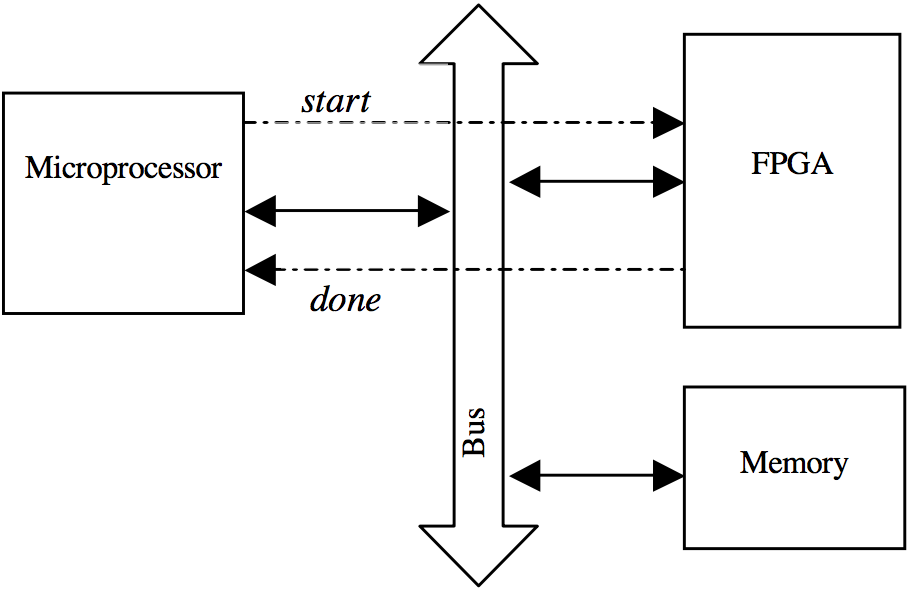
\includegraphics[width=0.7\textwidth]{img/into-soc.png}
        \caption{Visão geral de um SoC FPGA.}
        \label{fig:rb-soc}
    \end{figure}
    
    \pdfnote{HC: um pedaço de CI dentro (ou não) de um FPGA}
    \pdfnote{SC: é obtido por meio de \design\ e sintetização na placa }
    \pdfnote{vantags:}
    \pdfnote{usar todos recursos, máxima performance}
    \pdfnote{permite a extensão da arquitetura}
    \pdfnote{-> HDL}
    \end{frame}
